\chapter{Le contexte de résolution du problème}
\chaptermark{Contexte}
\minitoc
\newpage
 
\section{Le problème à résoudre} 
Bien que la recommandation aujourd'hui soit le moyen efficace d'améliorer non seulement la connaissance client mais aussi bien ciblé ses clients, elle pose des problèmes dans sa mise en place. 
Les grandes difficultés confrontées dans la mise en place des modèles de recommandation:
\begin{enumerate}
\item L’information sur l’avis client:\\
L’avis du client sur un produit donné peut être explicite soit direct ou implicite. L’avis explicite c’est des formes de likes, votes sur les préférences que le client attribue à un produit après l’avoir testé. Le problème à ce niveau est que peu de clients font des retours d’expérience sur le produits, par conséquent moins d’information pour construire un bon modèle de recommandation.\\
D’un autre côté on dispose des informations implicites que le client donne en faisant l’analyse de son comportement. C’est l’exemple du temps passé sur une page, les types d’articles qui ont plus de clics… Les avis implicites sont faciles à collecter en masse car ils ne demandent pas d’effort du côté client. Mais, le problème ici aussi est que ces avis implicites ne renseignent pas effectivement l'intérêt ou non du client à un article. La présence des avis implicite des clients en abondance ont permis de faire beaucoup de recherche dans l’amélioration des modèles de recommandation.  

\item Manque d’avis clients en comparaison au nombre d’article à recommander:\\
On dispose en majorité peu de données sur le vote et les avis clients en rapport avec le nombre produit présent dans la catalogue. 

\item Biais de popularité: non diversité des produits recommandés\\
En effet, l'objectif d'un système de recommandation est d'avoir moins de suggestion en haut de la liste recommandée, et induire plus de diversité dans cette liste recommandée. Par contre certains articles nouveaux par faute de popularité auront moins de chance de faire partie de la liste alors qu’ils pourraient potentiellement intéresser le client.
\end{enumerate}

Le problème à résoudre dans ce mémoire sera d’appliquer des modèles de recommandation au secteur du vélo. Les données sont essentiellement des votes que les clients attribuent à chaque pièce de vélo lors de l’achat.


\newpage
\section{Présentation des données}
\subsection{Dataset:}
Les données à étudier contiennent des informations de chaque article avec le vote, l’avis, … que le client lui a attribué. Ces données sont issues du scrapping des sites des fournisseurs. Elle contient actuellement 30.912 lignes et 11 colonnes.
\begin{figure}[h]
\begin{center}
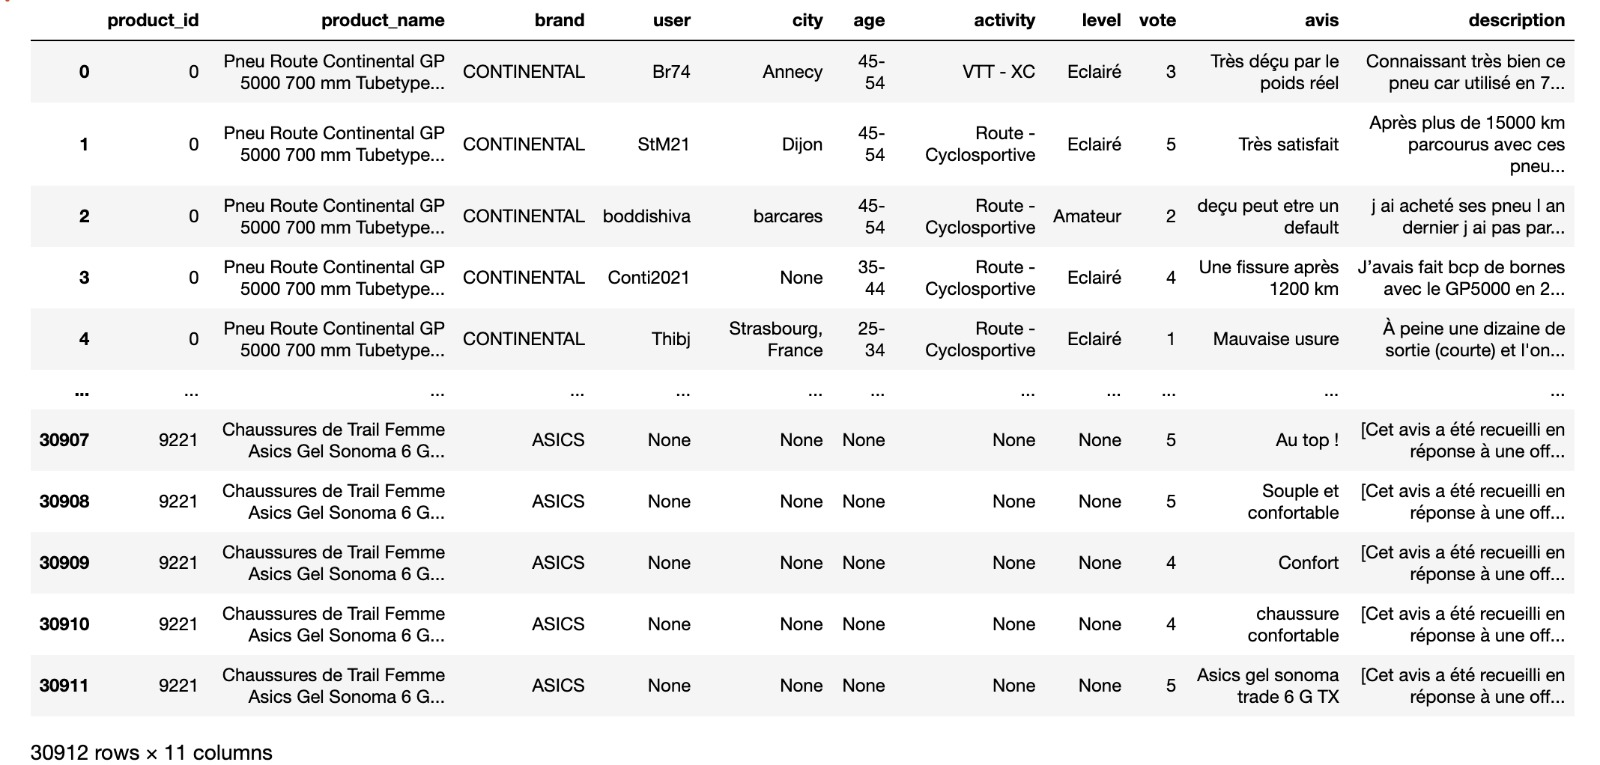
\includegraphics[width=15cm,height=6cm]{images/sample_data.jpeg}
\caption[Jeu de donnée]{Jeu de donnée}
\label{monlabel}
\end{center}
\end{figure}

\begin{figure}[h]
\begin{center}
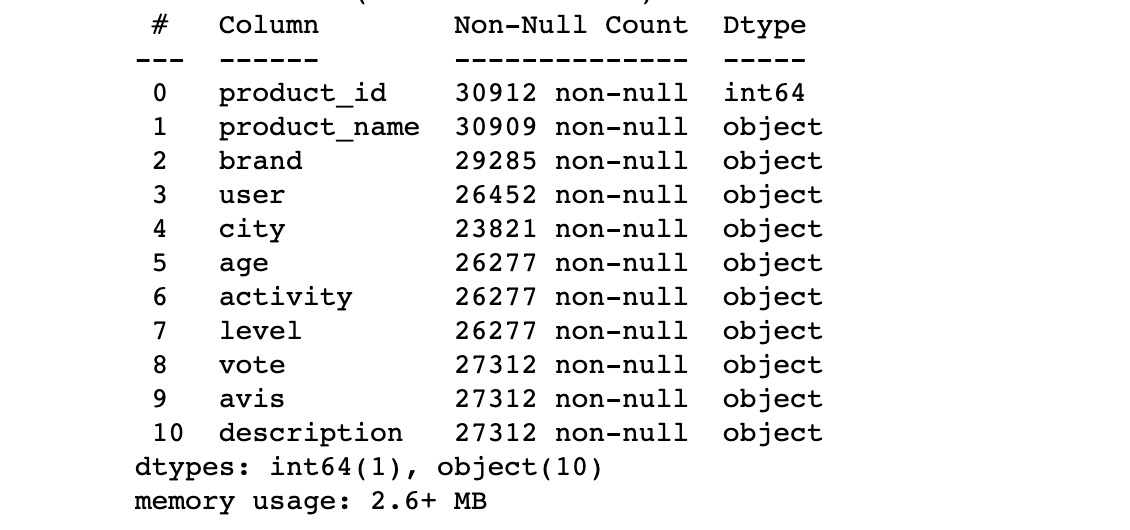
\includegraphics[width=15cm,height=6cm]{images/detail_columns.jpeg}
\caption[Détail des colonnes]{Détail des colonnes}
\label{monlabel}
\end{center}
\end{figure}

\subsection{Détail des colonnes de la dataset:}
\begin{itemize}
  	\item product name: Nom du produit que le client a acheté
	\item brand: la marque du produit 
	\item user: représente le nom du client
	\item city: la ville où habite le client, 
	\item age: la tranche d'âge du client, elle peut nous être à identifier pour chaque produit la tranche d'âge d’individus qui s’y intéressent.
	\item activity: le type d’activité que le client effectue avec son vélo (Compétition, Voyage, …)
	\item level: le niveau atteint dans son activité dans la pratique du vélo,
	\item vote: le score attribué au produit acheté sur le site
	\item avis: défini le sentiment que porte le client à l’issue de l’achat de l’article,
	\item description: le commentaire que porte le client sur le produit acheté.
\end{itemize}

\newpage
\section{Méthodes de validation des modèles}
\subsection{MSE: Mean Squared Error ou RMSE: Root Mean Squared Error}
Le Mean Squared Error est une fonction mathématique permettant d’évaluer la performance d’un modèle ayant des valeurs de prédiction continues. C’est la moyenne des erreurs au carré de tous les points de données d’apprentissage ou de validation. 
Supposons un vecteur de n prédictions noté Y d’un modèle à partir d’une matrice de n donnée X.
Le MSE est donné par la formule suivante:
$$
\mathrm{MSE}=\frac{1}{n} \sum_{i=1}^n\left(Y_i-\hat{Y}_i\right)^2
$$
Le RMSE est donné par la formule suivante:
$$
\mathrm{RMSE}=\sqrt{\frac{1}{n} \sum_{i=1}^n\left(Y_i-\hat{Y}_i\right)^2}
$$
En fonction de l'époque, le modèle apprend en s’améliorant lorsque le MSE converge vers 0.

\subsection{MAE: Mean Absolute Error}
Le Mean Absolute Error est une fonction mathématique permettant d’évaluer la performance d’un modèle ayant des valeurs de prédiction continues. 
C’est la moyenne de la différence absolue entre la prédiction et les valeurs réelles.
Sa formule est donnée par:
$$\mathrm{MAE}=\frac{1}{n} \sum_{j=1}^n\left|y_j-\hat{y}_j\right|
$$
Sa valeur décroît en fonction de l'époque d’apprentissage.
\begin{figure}[h]
\begin{center}
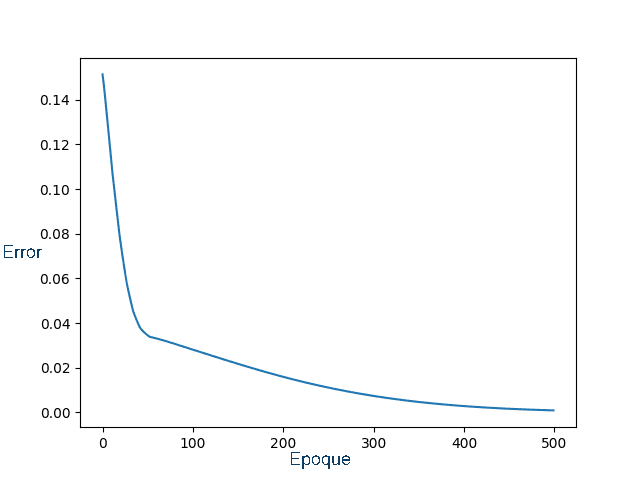
\includegraphics[width=15cm,height=8cm]{images/error_evaluation.png}
\caption[Allure de l'evolution de l'erreur en fonction de l'époque]{Allure de l'evolution de l'erreur en fonction de l'époque}
\label{monlabel}
\end{center}
\end{figure}





